\documentclass{standalone}

\usepackage{tikz}
\usepackage{standalone}
\usetikzlibrary{calc}
\usepackage{pgfplots}
\usepackage{color}

\begin{document}

    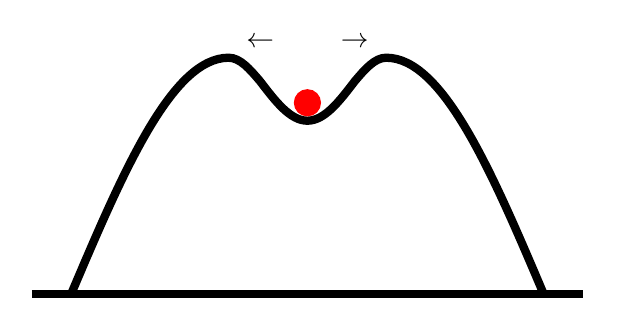
\begin{tikzpicture}

    \draw[-, line width=3pt] (-1.5, 0) -- (5.5, 0) node[right] {};

    \draw[line width=3pt] (-1, 0) sin (1, 3) cos (1.4, 2.7) sin (2, 2.2) cos (2.6, 2.7)
    sin(3, 3) cos(5, 0);

    \node[circle, red, draw, fill] (0) at (2, 2.428) {};

    \node (1) at (2.6, 3.2) {$\rightarrow$};
    \node (2) at (1.4, 3.2) {$\leftarrow$};
    \end{tikzpicture}

\end{document}